\documentclass[10pt]{beamer}

\usepackage[utf8]{inputenc}
\usepackage[spanish, es-tabla]{babel}

\usetheme{metropolis}
\usepackage{appendixnumberbeamer}

\usepackage{booktabs}
\usepackage[scale=2]{ccicons}

\usepackage{pgfplots}
\usepgfplotslibrary{dateplot}

\usepackage{caption}
\usepackage{subcaption}

\usepackage{graphicx}

\usepackage{amsmath}
\usepackage{amsfonts}
\usepackage{amssymb}
\usepackage{amsthm}
\usepackage{esvect}

\usepackage{multimedia}

\usepackage{xspace}
\newcommand{\themename}{\textbf{\textsc{metropolis}}\xspace}

\title{Detección de anomalías basada en técnicas de ensembles}
\author{Ignacio Aguilera Martos}
\date{\today}
\institute{Trabajo Fin de Grado \\ \href{https://github.com/nacheteam/Ensemble-Outlier-Analysis}{Código disponible en GitHub}}

\begin{document}

\maketitle

\begin{frame}[fragile]{Contenidos}
  \setbeamertemplate{section in toc}[sections numbered]
  \tableofcontents[hideallsubsections]
\end{frame}

\section{Concepto de anomalía basado en distancias}

\begin{frame}[fragile]{Tukey's Fences}
\vspace{10px}
\pause
\metroset{block=fill}

Pensado para el caso uno-dimensional.

\pause

\begin{block}{Tukey's Fences}
	Valores fuera del rango $[Q_1 - k(Q_3 - Q_1), Q_3 + k(Q_3 - Q_1)]$ con $k=1.5$
\end{block}

\pause

La propuesta de $k=1.5$ es arbitraria.

\end{frame}

\begin{frame}[fragile]{Tukey's Fences}
\vspace{10px}
\metroset{block=fill}
\centering
\movie[height = 0.8\textheight, width=0.8\textwidth, poster, showcontrols]{}{Imagenes/outlier-1d.mp4}

\end{frame}

\begin{frame}[fragile]{Tukey's Fences}
\vspace{10px}
\metroset{block=fill}

\begin{figure}
	\centering
	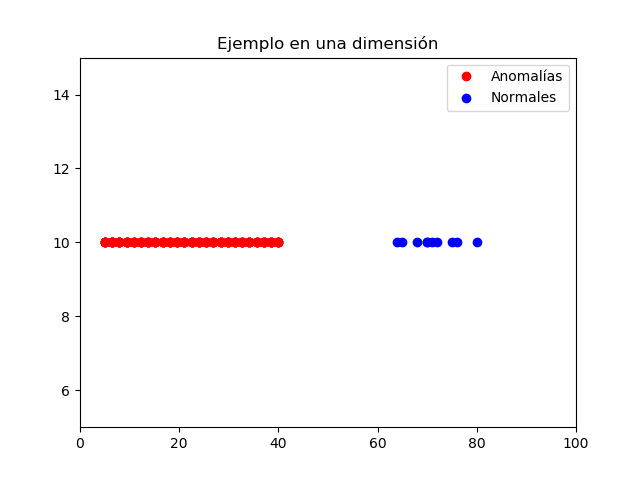
\includegraphics[scale=0.6]{Imagenes/outlier-1d.png}
\end{figure}

\end{frame}

\begin{frame}[fragile]{Extensión al caso de mayor dimensionalidad}
\vspace{10px}
\pause
\metroset{block=fill}

\begin{block}{Criterio}
	Aplicar el criterio de Tukey a cada una de las características.
	\pause
	\textbf{\underline{Trivial}}.
\end{block}

\pause

\begin{block}{Criterio de clusters}
	\begin{enumerate}
		\item Agrupamos los datos por clusters.
		\pause
		\item Encontramos el cluster más cercano para cada instancia.
		\pause
		\item Si la distancia del objeto al centroide del cluster es mayor que $1.5$ veces la mayor
		distancia intercluster entonces es una anomalía.
	\end{enumerate}
\end{block}

\end{frame}

\begin{frame}[fragile]{Ejemplo 1}
\vspace{10px}
\metroset{block=fill}
\centering
\movie[height = 0.8\textheight, width=0.8\textwidth, poster, showcontrols]{}{Imagenes/outlier-2d-case1.mp4}

\end{frame}

\begin{frame}[fragile]{Ejemplo 1}
\vspace{10px}
\metroset{block=fill}

\begin{figure}
	\centering
	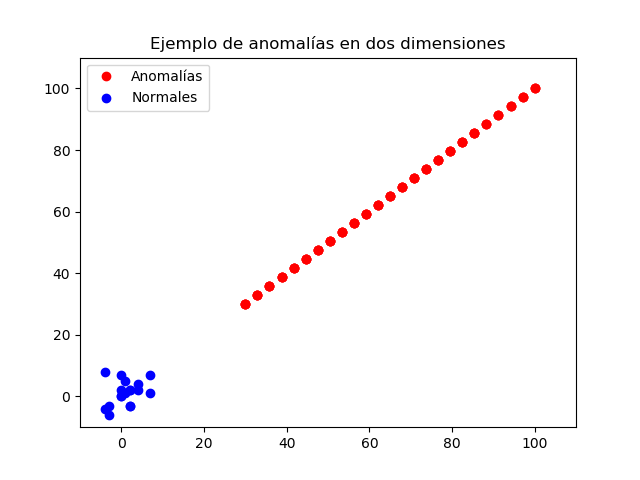
\includegraphics[scale=0.6]{Imagenes/outlier-2d-case1.png}
\end{figure}

\end{frame}

\begin{frame}[fragile]{Ejemplo 2}
\vspace{10px}
\metroset{block=fill}
\centering
\movie[height = 0.8\textheight, width=0.8\textwidth, poster, showcontrols]{}{Imagenes/outlier-2d-case2.mp4}

\end{frame}

\begin{frame}[fragile]{Ejemplo 2}
\vspace{10px}
\metroset{block=fill}

\begin{figure}
\centering
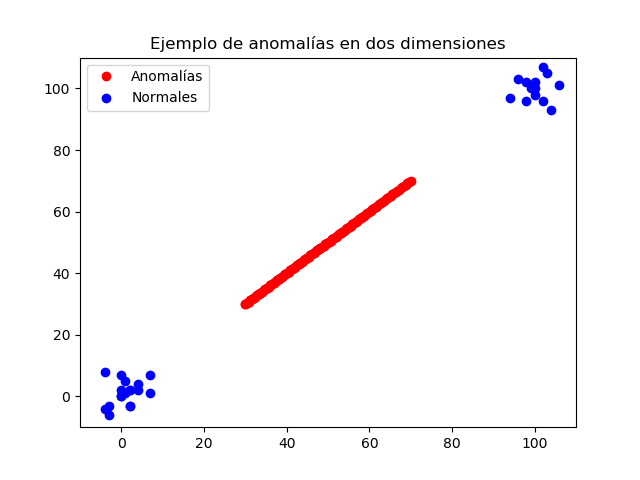
\includegraphics[scale=0.6]{Imagenes/outlier-2d-case2.png}
\end{figure}

\end{frame}

\section{Aprendizaje Automático}

\begin{frame}[fragile]{Problema que abordamos}
\vspace{10px}
\pause
\metroset{block=fill}

\begin{alertblock}{Problema de detección de anomalías}
	Es un problema de aprendizaje no supervisado pues no disponemos de las etiquetas.
\end{alertblock}

\pause

\begin{block}{Partes teóricas del problema}
	\begin{enumerate}
		\item Generador.
		\item Sistema.
		\item Máquina de aprendizaje.
	\end{enumerate}
\end{block}

\end{frame}

\begin{frame}[fragile]{Alta dimensionalidad}
\vspace{10px}
\pause
\metroset{block=fill}

\begin{block}{Propiedades de conjuntos de alta dimensionalidad}
	\begin{enumerate}
		\item La densidad disminuye exponencialmente al aumentar la dimensionalidad.
		\pause
		\item Cuanto mayor es la dimensionalidad mayor debe ser el radio de una bola para englobar el mismo porcentaje de datos.
		\pause
		\item Casi todo punto está más cerca del borde del conjunto que de otro punto. 
		$$D(d,n) = (1-\frac{1}{2}^{\frac{1}{n}})^{\frac{1}{d}}$$
		\pause
		\item Casi todo punto es una anomalía sobre su propia proyección.
	\end{enumerate}
\end{block}

\pause

\begin{alertblock}{Maldición de la alta dimensionalidad}
	A mayor dimensionalidad mayor número de puntos necesitamos para obtener una aproximación con funciones de igual regularidad.
\end{alertblock}

\end{frame}

\begin{frame}[fragile]{Aproximación de funciones}
\vspace{10px}
\pause
\metroset{block=fill}

\begin{alertblock}{Aproximación de funciones}
	Nuestro objetivo es aproximar la función de salida del sistema con los datos que tenemos.
\end{alertblock}

\pause

\begin{block}{Teoremas útiles}
	\begin{itemize}
		\item Teorema de Aproximación de Weierstrass
		\pause
		\item Serie de Fourier
		\pause
		\item Teorema de Kolmogorov-Arnold
	\end{itemize}
\end{block}

\end{frame}

\begin{frame}[fragile]{Teorema de Aproximación de Weierstrass}
\vspace{10px}
\pause
\metroset{block=fill}

\begin{block}{Teorema de Aproximación de Weierstrass}
	Supongamos que tenemos una función $f:[a,b]\rightarrow \mathbb{R}$ continua. Entonces $\forall \epsilon > 0$ existe un polinomio $p$ tal que $\forall x \in [a,b]$ tenemos que $|f(x)-p(x)|<\epsilon$.
\end{block}

\pause

\begin{alertblock}{Aproximación por polinomios}
	El Teorema de Aproximación de Weierstrass nos da una forma de aproximar funciones por polinomios.
\end{alertblock}

\end{frame}

\begin{frame}[fragile]{Serie de Fourier}
\vspace{10px}
\pause
\metroset{block=fill}

\begin{block}{Serie de Fourier}
	Si tenemos una función $f:\mathbb{R} \rightarrow \mathbb{R}$ integrable en el intervalo $[t_0 - \frac{T}{2}, t_0 + \frac{T}{2}]$ entonces se puede obtener el desarrollo de Fourier de $f$ en dicho intervalo. Si $f$ es periódica en toda la recta real la aproximación es válida en todos los valores en los que esté definida.
	
	$$f(t) \approx \frac{a_0}{2} + \sum_{n=1}^{\infty}\left[ a_n \cos (\frac{2n\pi}{T}t) + b_n \sin (\frac{2n\pi}{T}t) \right]$$
	
	$$a_0 = \frac{2}{T}\int_{-\frac{T}{2}}^{\frac{T}{2}}f(t)dt, \ a_n = \frac{2}{T}\int_{-\frac{T}{2}}^{\frac{T}{2}} f(t) \cos (\frac{2n\pi}{T}t) dt,$$
	
	$$b_n = \frac{2}{T} \int_{-\frac{T}{2}}^{\frac{T}{2}} f(t) \sin (\frac{2n\pi}{T}t) dt$$
\end{block}

\end{frame}

\begin{frame}[fragile]{Teorema de Kolmogorov-Arnold}
\vspace{10px}
\pause
\metroset{block=fill}

\begin{block}{Teorema de Superposición Kolmogorov-Arnold}
	Sea $f$ una función continua de varias variables $f:X_1 \times ... \times X_n \rightarrow \mathbb{R}$, entonces existen funciones $\Phi_q : \mathbb{R}\rightarrow \mathbb{R}$ y $\phi_{q,p} : X_p \rightarrow [0,1]$ tales que $f$ se puede expresar como:
	
	$$f(x) = f(x_1, ..., x_n) = \sum_{q=0}^{2n}\Phi_q ( \sum_{p=1}^{n}\phi_{q,p}(x_p))$$
\end{block}

\pause

\begin{alertblock}{Dimensionalidad en datos y funciones}
	La maldición de la dimensionalidad es intrínseca a los datos. Este Teorema nos dice que la capacidad expresiva o complejidad de las funciones de una sola variable es la misma que las de varias variables.
\end{alertblock}

\end{frame}

\begin{frame}[fragile]{Equilibrio Sesgo-Varianza}
\vspace{10px}
\pause
\metroset{block=fill}

\begin{block}{Notación}
	$$MSE = \frac{1}{n}\sum_{i=1}^{n}{y_i - g(X_i,\mathcal{D})}^2$$
	
	$$E[MSE] = \frac{1}{n}\sum_{i=1}^{n}E[{y_i - g(X_i,\mathcal{D})}^2] = \cdots$$
	
	$$ = \frac{1}{n}\sum_{i=1}^{n}\{ f(X_i) - E[g(X_i, \mathcal{D})] \}^2 + \frac{1}{n}\sum_{i=1}^{n}E[\{ E[g(X_i, \mathcal{D})] - g(X_i, \mathcal{D}) \}^2]$$
	
	$$ = sesgo^2 + varianza$$
\end{block}

\end{frame}

\begin{frame}[fragile]{Teoría del Aprendizaje}
\vspace{10px}
\pause
\metroset{block=fill}

\begin{block}{Teorema clave de la Teoría del Aprendizaje}
	Para funciones de pérdida acotadas el principio inductivo de minimización del error empírico es consistente sí y sólo si el error empírico converge uniformemente al valor real del error en el siguiente sentido:
	
	$$\lim\limits_{n\rightarrow \infty} P[\sup_{\omega}|R(\omega) - R_{emp}(\omega)|>\epsilon] = 0 \ , \ \forall \epsilon >0$$
\end{block}

\end{frame}

\begin{frame}[fragile]{Cota ERM}
\vspace{10px}
\pause
\metroset{block=fill}

\begin{block}{Dimensión VC}
	Decimos que un conjunto de funciones tiene dimensión VC $h$ si puede resolver de forma óptima todos los casos de tamaño $h$ pero existe al menos uno de tamaño $h+1$ que no puede resolver.
\end{block}

\pause

\begin{block}{Cota ERM}
	Con probabilidad $1-\eta$
	
	$$R(\omega) \leq R_{emp}( \omega) + \frac{\epsilon}{2} \biggl( 1+\sqrt{1+\frac{4\cdot R_{emp}(\omega)}{\epsilon}} \biggl)$$
	
	\pause
	
	$$\epsilon = a_1 \cdot \frac{h(\ln (\frac{a_2 n}{h})+1) - \ln (\frac{\eta}{4})}{n}$$
\end{block}

\end{frame}

\section{Probabilidad Multivariante}

\begin{frame}[fragile]{Contenidos de la sección}
\vspace{10px}
\pause
\metroset{block=fill}

\begin{block}{Contenidos útiles}
	\begin{itemize}
		\item Vectores aleatorios.
		\pause
		\item Independencia.
		\pause
		\item Probabilidad condicionada (sucesos, variables y $\sigma$-álgebras) y sus propiedades.
		\pause
		\item Esperanza condicionada (sucesos, variables y $\sigma$-álgebras) y sus propiedades.
		\pause
		\item Desigualdades famosas.
	\end{itemize}
\end{block}

\end{frame}

\begin{frame}[fragile]{Desigualdad de Markov y Chebychev}
\vspace{10px}
\pause
\metroset{block=fill}

\begin{block}{Desigualdad de Markov}
	Sea $X$ una variable aleatoria que toma valores no negativos. Entonces para cualquier constante $\alpha$ satisfaciendo $E[X]<\alpha$ se cumple que:
	
	$$P(X>\alpha)\leq \frac{E[X]}{\alpha}$$
\end{block}

\begin{block}{Desigualdad de Chebychev}
	Sea $X$ una variable aleatoria arbitraria. Entonces para cualquier constante $\alpha$ se tiene que:
	
	$$P(|X - E[X]|>\alpha)\leq \frac{Var[X]}{\alpha^2d}$$
\end{block}

\end{frame}

\begin{frame}[fragile]{Desigualdades famosas}
\vspace{10px}
\pause
\metroset{block=fill}

\begin{block}{Desigualdades estudiadas}
	\begin{itemize}
		\item Desigualdad de Markov
		\item Desigualdad de Chebychev
		\item Cotas de Chernoff
		\item Desigualdad de Hoeffding
	\end{itemize}
\end{block}

\end{frame}

\section{Concepto probabilístico de anomalía}

\begin{frame}[fragile]{Notación}
\vspace{10px}
\pause
\metroset{block=fill}

\begin{block}{Notación usada}
	$$X = \{ x_1 , ... , x_n \}, \ x_i = (x_{s_1} , ... , x_{s_d})$$
	
	\pause
	
	$$S = \{ s_i | s_i \in \{ s_1 , ... , s_d \} \ con \ i\in \Delta \}$$
	
	\pause
	
	$$X_S \ proyecci\acute{o}n \ de \ los \ datos \ en \ el \ subespacio \ S$$
	
	\pause
	
	$$p_{s_1 , ... , s_p}(x_{s_1} , ... , x_{s_p})$$
	
	\pause
	
	$$p_{s_i}(x_{s_i})$$
\end{block}

\end{frame}

\begin{frame}[fragile]{Definiciones}
\vspace{10px}
\pause
\metroset{block=fill}

\begin{block}{Definición subespacio incorrelado}
	Decimos que un subespacio $S$ es un subespacio incorrelado si y sólo si:
	
	$$p_{s_1 , ... , s_p}(x_{s_1} , ... , {x_{s_p}}) = \prod_{i=1}^{p}p_{s_i}(x_{s_i})$$
\end{block}

\pause

\begin{block}{Definición anomalía no trivial}
	Decimos que un objeto $x_S$ es una anomalía no trivial respecto del subespacio $S$ si:
	
	$$p_{s_1 , ... , s_p}(x_{s_1} , ... , x_{s_p})\ll p_{esp}(x_{s_1} , ... , x_{s_p})$$
\end{block}

\pause

\begin{alertblock}{Relación entre conceptos de anomalía}
	Este concepto de anomalía es complementario.
\end{alertblock}

\end{frame}

\begin{frame}[fragile]{Ejemplo de anomalía}
\vspace{10px}
\pause
\metroset{block=fill}

\begin{figure}
	\centering
	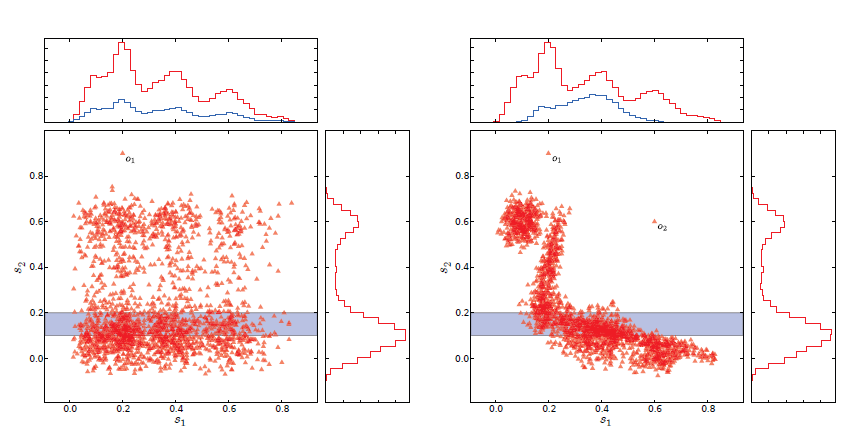
\includegraphics[scale=0.5]{Imagenes/ejemplo_anomalia_probabilidad}
\end{figure}

\end{frame}

\begin{frame}[standout]
	\LARGE{¿Preguntas?}
	\vspace{10px}
\end{frame}


\end{document}
